\chapter{Felhasználói dokumentáció} % User guide
\label{ch:user}



% SW purpose
\section{A Szoftver Célja} 

A szoftver egy SHA-256 algoritmussal hash-elt jelszavak feltörésére alkalmas C++ és OpenCL-ben írt program. A célja a modern videókártya használat hatásának vizsgálata a jelszófeltörés sebességére nézve. Jelenleg a program képes videokártya használatával hash-elni egy jelszót, egy fájl megadásával hashelni több jelszót, vagy feltörni egy általános, vagy salt-al ellátott jelszót, amennyiben az szerepel a megadott ismert jelszavak listában. Ezt a feladatát speciálisan a használt rendszerre optimalizálva teszi.

A programot biztonságtechnikai kutatóknak, vagy diákoknak javaslom, akik érdekeltek abban, hogy milyen sebességgel törhető fel egy biztonságosnak számító jelszó a számukra elérhető hardverekkel.


\section{A Szoftver Használata}


%System requirements
\subsection{Rendszerkövetelmények}

A program Microsoft Windows operációs rendszeren futtatható exe formájában érhető el.

\begin{table}[H]
    \begin{tabular}{|l|l|l|}
        \hline
        & Minimális  & Optimális (vagy újabb/jobb) \\
        \hline
        Operációs Rendszer & Microsoft Windows 7 & Microsoft Windows 10 \\
        \hline
        Videókártya  & OpenCL-t támogató   & \begin{tabular}[c]{@{}l@{}}NVidia GeForce GTX 600-as széria\\
                                                            AMD Radeon R9/ HD 7000 széria
                                             \end{tabular}\\
        \hline
        Háttértár & 7200 RPM HDD & M.2 PCIe SSD \\
        \hline
    \end{tabular}
    \caption{A program rendszerkövetelményei.}
\end{table}


%Installation
\subsection{Telepítés}

A program letöltése után egy zip állomány áll a rendelkezésre. Ezt az állomány kell kicsomagolni egy erre alkalmas programmal (például 7-Zip) és a benne található mappát egy megfelelő helyre helyezni. Fontos, hogy a mappában található fájlok mindegyike továbbra is azonos mappában helyezkedjen el, ezen kívül bárhová helyezhető a számítógépen, ahol ön rendelkezik olvasási és futtatási joggal.

A program futtatása a konzolon keresztül a fájlokat tartalmazó mappából történik, ezért érdemes kényelmes elérést biztosítani a fájlhoz. Erre egy jó módszer lehet például az alapértelmezett C meghajtó gyökérkönyvtárába helyezni a mappát, amely a következő helyen elérhető lesz: C:\textbackslash gpucrack\textbackslash



%Contols
\subsection{Vezérlés}

A szoftver konzolos felületen indítási paraméterek megadásával konfigurálható. A szoftvert tartalmazó mappában megnyitott konzol ablakban a következő paranccsal tudjuk futtatni a programot (.\textbackslash sha256gpu.exe). Ekkor angol nyelven a program felsorolja a használható parancsokat, amelyek közül választhatunk:
%
\begin{itemize}
    \item platform - Felsorolja az elérhető platformokat és eszközöket.
    \item hash single <password> - Hash-el egy jelszót, majd kiírja az eredményt.
    \item hash single <password> <salt> - Hash-el egy jelszót egy salt-al együtt, majd kiírja az eredményt.
    \item hash multiple <source> <target> - Első paraméterként egy enterrel elválasztott kulcsokkal teli fájlt adhatunk meg, amely mindegyikét hashelni és enterrel elválasztva a target-nek meghatározott fájlba írja.
    \item crack single <source> <hash> - A megadott hash kódot megpróbálja a passwords fájlban található jelszavak segítségével feltörni. Amennyiben sikerül, kiírja az eredeti kulcsot, ellenkező esetben jelzi, hogy nem talált megfelelő kulcsot.
\end{itemize}

\noindent Ezek mellett minden parancsnak megadhatunk egy kapcsolót.
%
\begin{table}[H]
\centering
    \begin{tabular}{|l|l|l|}
        \hline
        Kapcsoló                          & Alapértelmezett & Hatás                                          \\
        \hline
        -p \textless{}id\textgreater{}    & 0                     & A használt platform kiválasztása               \\
        \hline
        -d \textless{}id\textgreater{}    & 0                     & A használt eszköz kiválasztása                 \\
        \hline
        -t \textless{}count\textgreater{} & 1024                  & Egyszerre feltörhető jelszavak száma \\
        \hline
        -k \textless{}size\textgreater{}  & 24                    & Egy bemeneti kulcs maximális mérete \\
        \hline
    \end{tabular}
    \caption{A programban használható kapcsolók leírása}
\end{table}

Minden kapcsoló használata opcionális, azonban a -t kifejezetten fontos az optimális sebesség elérésének érdekében, amelyet egy néhány teszt futtatással finomhangolni lehet. A -p és -d kapcsolók kizárólag akkor relevánsak, ha nem az alapértelmezett eszközt használjuk feltörésre. A kulcs maximális méretének csökkenése egy minimális teljesítmény növekedést eredményezhet, amennyiben ismert hogy, a maximum használt jelszó mérete például 16 volt és a mintadokumentum kizárólag ekkora vagy, ennél rövidebb jelszavakat tartalmaz.

\begin{figure}[H]
    \centering
    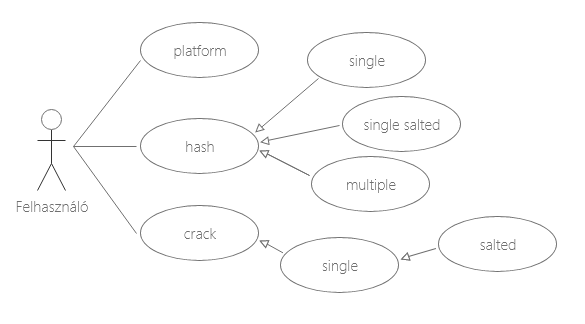
\includegraphics[width=\textwidth]{images/diagrams/use-case.png}
    \caption{Use-case diagram.}
    \label{fig:use-case}
\end{figure}





%Input
\subsection{Bemenet}

A bemeneti értékek minden parancsra különböznek, azonban ezek kategóriákra oszthatóak.
%
\begin{itemize}
    \item <password> jelszó: egy karaktersorozat, amely kizárólag az UTF-8 táblázat elemeit tartalmazhatja
    \item <salt> salt: a követelmény megegyezik a jelszóéval
    \item <source> fájl: egy fájlt egyértelműen meghatározó elérési útvonal. Lehet abszolút és relatív. A fájl tartalmának ASCII, vagy utf-8 karaktereknek kell lennie, amelyeket sortörés karakterek választanak el egymástól.
    \item <target> fájl: egy fájlt egyértelműen meghatározó elérési útvonal. Lehet abszolút és relatív. A fájl vagy nem létezik (a mappában kell rendelkezni írási joggal), vagy írható (a régi fájl felülírásra kerül). Ha a mappa nem írható az ön felhasználói profiljából, indítsa a programot rendszergazdaként!
    \item <hash> hash: 64 hexadecimális (0-9, a-f) karaktert tartalmazó szöveg. Amennyiben salt-al rendelkezik, azok a karakterek a hash előtt helyezkednek el hozzáfűzve ahhoz. Ilyen esetben lehet hosszabb a szöveg mint 64 karakter.
\end{itemize}
%
Amennyiben a program hibát észlel a bemenetekkel, azonnal megszakítja a futást és a felhasználó tudtára adja, hogy mi okozta azt.






%Output
\subsection{Kimenet}

A program a kimenetet többnyire az azt elindító konzolos ablakba írja. Ezzel együtt minden esetleges hibaüzenet, vagy sikertelen futás eredménye is oda kerül. A kimenetek ezen felül tartalmaznak részletes információt például a megkapott hash felbontásáról és a futásidőről.
%
\begin{itemize}
    \item platform: a számítógépen található platformok és eszközök listája
    \item hash sinle: a megadott jelszó, vagy jelszó és salt sha256 hash alakja
    \item hash multiple: a megadott jelszófájl jelszavainak a sha256 hash-jei a target fájlban.
    \item crack single: amennyiben sikeres volt a feltörés a hash-hez tartozó jelszó és egyéb információk, amennyiben nem volt sikeres, akkor ezt kiírja a felhasználónak.
\end{itemize}





%Examples
\subsection{Példák}

Paraméter nélküli indítás:
%
\begin{figure}[H]
    \centering
    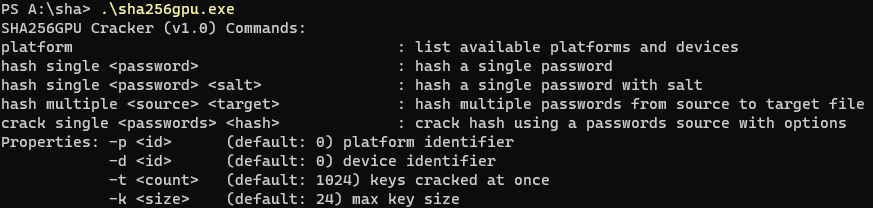
\includegraphics[width=\textwidth]{images/examples/example-empty.png}
\end{figure}

Számítási hardware-platformok kiíratása:
%
\begin{figure}[H]
    \centering
    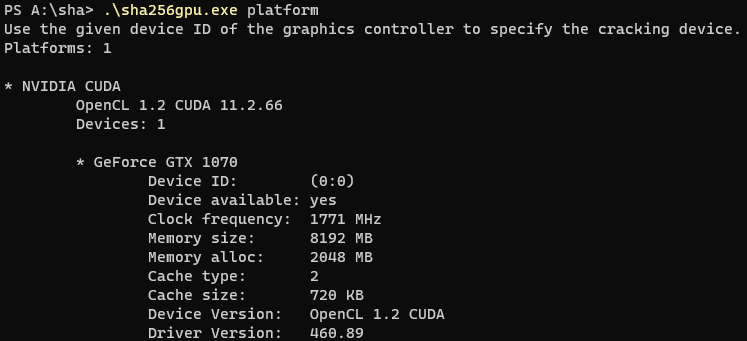
\includegraphics[width=\textwidth]{images/examples/example-platform.png}
\end{figure}

Hash kiszámítása:
%
\begin{figure}[H]
    \centering
    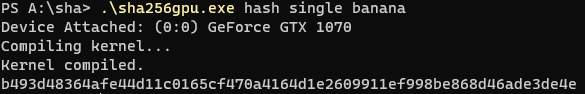
\includegraphics[width=\textwidth]{images/examples/example-hash.png}
\end{figure}

Jelszó sikeres feltörése:
%
\begin{figure}[H]
    \centering
    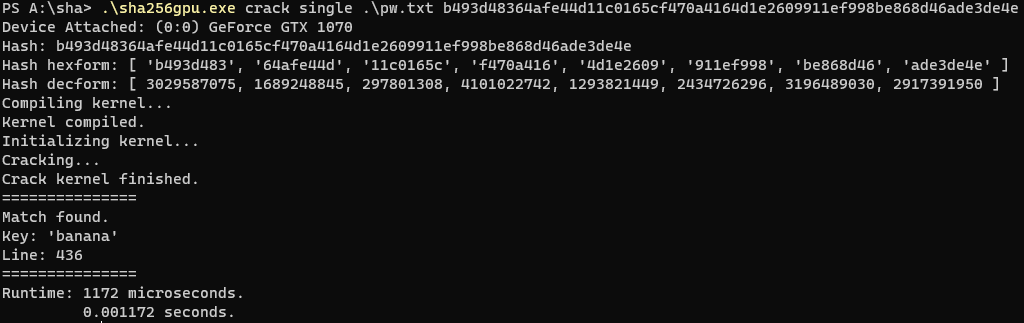
\includegraphics[width=\textwidth]{images/examples/example-crack.png}
\end{figure}

Jelszó sikertelen feltörése:
%
\begin{figure}[H]
    \centering
    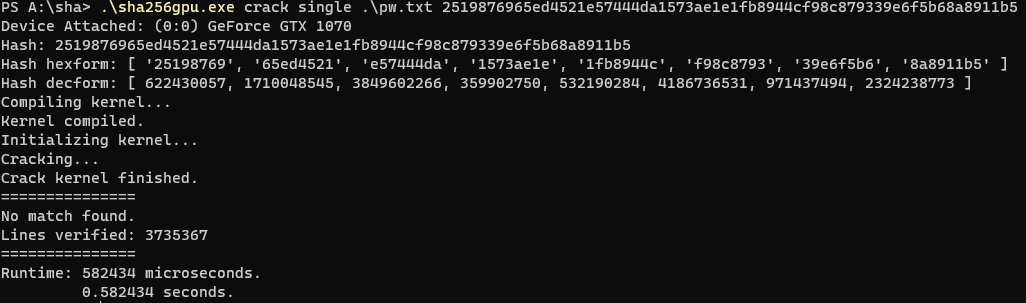
\includegraphics[width=\textwidth]{images/examples/example-crack-unsuccessful.png}
\end{figure}

Jelszó paraméterezett feltörése:
%
\begin{figure}[H]
    \centering
    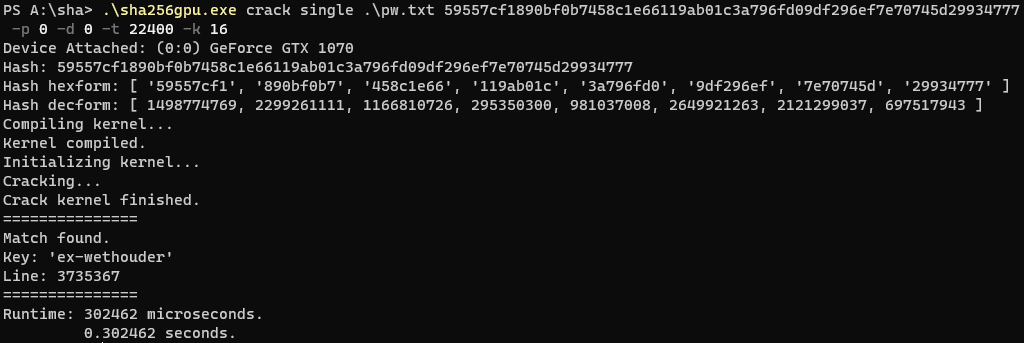
\includegraphics[width=\textwidth]{images/examples/example-crack-params.png}
\end{figure}

Jelszavak hashelése kimeneti fájlba:
%
\begin{figure}[H]
    \centering
    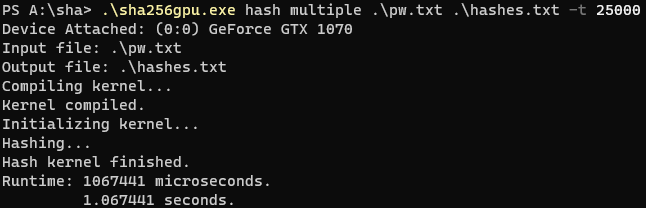
\includegraphics[width=\textwidth]{images/examples/example-hash-multiple.png}
\end{figure}

Jelszó és hash-fájlok tartalma (bal: bemenet, jobb: kimenet):
%
\begin{figure}[H]
    \centering
    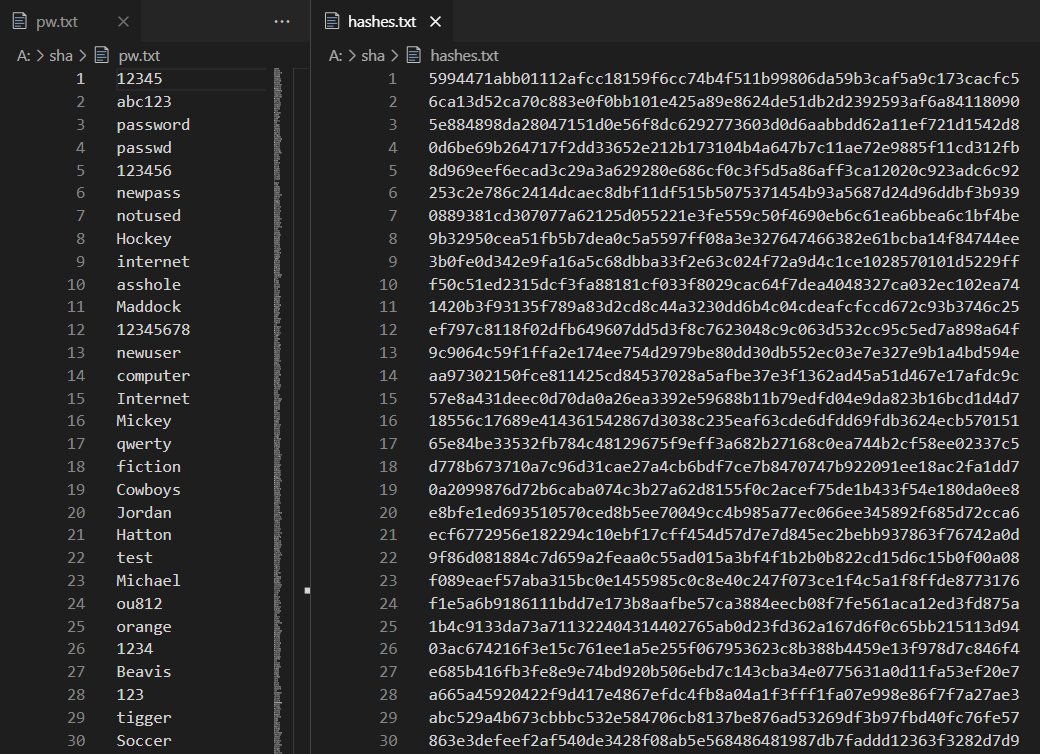
\includegraphics[width=\textwidth]{images/examples/example-hash-files.png}
\end{figure}


\subsection{Hiba Esetén}

A program hiba esetén leáll és leírással próbálja segíteni a probléma diagnosztizálását. Amennyiben ismeretlen hiba történik, próbálja meg a következő lépéseket elvégezni:
%
\begin{enumerate}
    \item Ellenőrizze le, hogy a parancs megfelelő formátumú-e.
    \item Próbálja meg kapcsolók nélkül futtatni a programot.
    \item Indítsa el a programot a (platform) parancs segítségével és bizonyosodjon meg róla, hogy található legalább egy eszköz.
    \item Frissítse a használni kívánt eszközt a legújabb driver verzióra.
    \item Frissítse a C++ Runtime szolgáltatást a legújabb verzióra.
    \item Amennyiben fájlal dolgozik, bizonyosodjon meg róla, hogy az elérési út megfelelő, a fájlhoz van hozzáférése és az olvasható.
    \item Bizonyosodjom meg róla hogy az eredeti zip-ben tárolt fájlok mindegyike megtalálható a futtatható fájlal egy mappában.
    \item Futtassa a programot rendszergazdai jogosultsággal.
\end{enumerate}